\documentclass[12pt, a4paper]{article}
\usepackage{geometry}
\usepackage{hyperref}
\usepackage{listings}
\usepackage{xcolor}
\usepackage{tabularx}
\usepackage{graphicx}
\usepackage{float}
\usepackage{setspace}

\geometry{margin=0.8in}
\singlespacing

\hypersetup{
    colorlinks=true,
    linkcolor=black,
    filecolor=magenta,
    urlcolor=cyan,
}

\lstset{
    backgroundcolor=\color{gray!10},
    basicstyle=\ttfamily\small,
    numbers=left,
    numberstyle=\tiny,
    frame=single,
    breaklines=true,
}

\begin{document}

\title{Insight: Financial Report Analysis Engine - Progress Report}
\author{
    Group259 \\
    Wang Yixin 72512080 \\
    Zhang Jiajun 72510615 \\
    Wang Hongyuan 72510222
}
\date{\today}

\maketitle

\section{Project Background and Objectives}

With the rapid development of financial markets, the number and complexity of
financial research reports are increasing. Analysts and investors need to
quickly extract key information from a large number of reports to make informed
investment decisions. However, traditional manual reading methods are
inefficient and difficult to handle massive amounts of information.

In recent years, the development of large language models (LLM) and
retrieval-augmented generation (RAG) technology has provided new solutions for
financial report analysis. By combining the capabilities of vector retrieval
and large language models, intelligent analysis and question-answering for
financial reports can be achieved.

The core objective of the Insight: Financial Report Analysis Engine project is
to build a vertical domain RAG question-answering system that benchmarks the
NotebookLM experience, focusing on the analysis of long, information-dense
financial PDF reports, and providing page-level citation tracking.

Specific objectives include:
\begin{enumerate}
    \item Implement efficient parsing and processing of financial PDF reports
    \item Build high-quality vector indexes to support fast and accurate information
          retrieval
    \item Integrate local large language models to provide intelligent question-answering
          and analysis capabilities
    \item Implement page-level citation tracking to enhance the credibility of answers
    \item Establish a comprehensive evaluation system to ensure system performance
\end{enumerate}

\section{Project Technology Stack}

The project adopts the following technology stack:
\begin{itemize}
    \item \textbf{Frontend Framework}: Gradio
    \item \textbf{Backend Framework}: LlamaIndex v0.10+
    \item \textbf{Vector Database}: ChromaDB
    \item \textbf{Embedding Model}: BAAI/bge-m3
    \item \textbf{Large Language Model}: Qwen2.5-7B/72B (locally deployed via Ollama)
    \item \textbf{PDF Parsing}: PyMuPDF
    \item \textbf{Evaluation Framework}: RAGAS
\end{itemize}

\section{Completed Work}

\subsection{System Architecture Design}
The overall system architecture design has been completed, adopting a highly
cohesive, low-coupling modular design, consisting of four core components:
\begin{itemize}
    \item Data ingestion layer: Responsible for PDF parsing and chunking
    \item Retrieval and generation layer: Implements vector retrieval and hybrid
          retrieval, as well as answer generation
    \item Evaluation closed-loop layer: Implements RAGAS evaluation
    \item Interaction layer: Builds Gradio frontend
\end{itemize}

\subsection{Core Module Implementation}

\subsubsection{Data Ingestion Layer}
Implemented PDF report parsing and chunking functionality, supporting semantic
chunking to improve the accuracy of information retrieval.

\subsubsection{Retrieval and Generation Layer}
Implemented vector retrieval and hybrid retrieval functionality, integrated
RAPTOR tree-based summarization technology, improving the efficiency and
accuracy of retrieval.

\subsubsection{Evaluation Closed-loop Layer}
Integrated RAGAS evaluation framework, implementing comprehensive system
performance evaluation.

\subsubsection{Interaction Layer}
Built Gradio frontend, providing a user-friendly interactive interface.

\subsection{Environment Configuration}
Completed system environment configuration, successfully deployed and running
on Mac Studio (M3 Ultra).

\begin{figure}[H]
    \centering
    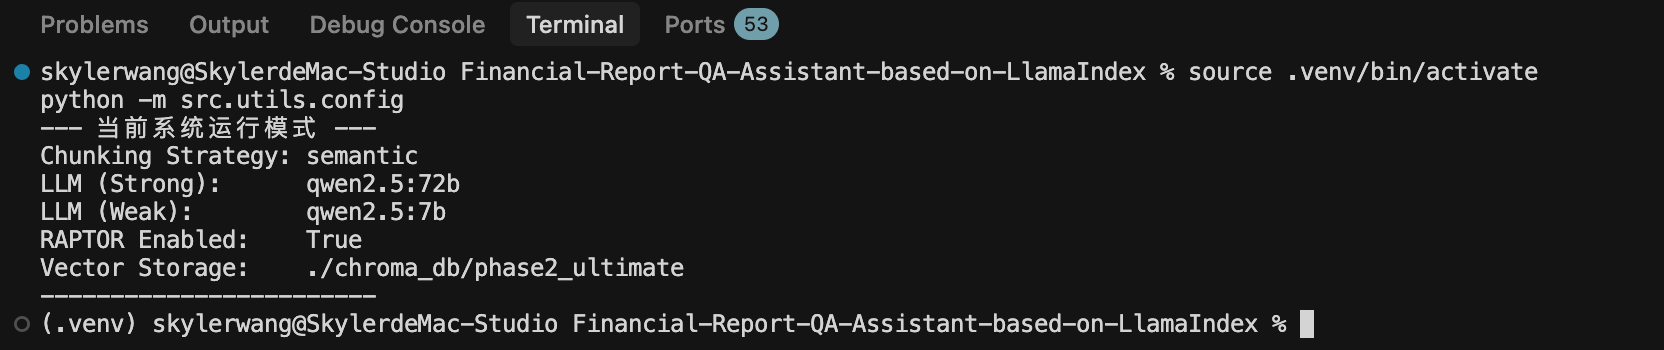
\includegraphics[width=0.6\textwidth]{../image/prompts/env.png}
    \caption{System Environment}
    \label{fig:environment}
\end{figure}

\begin{figure}[H]
    \centering
    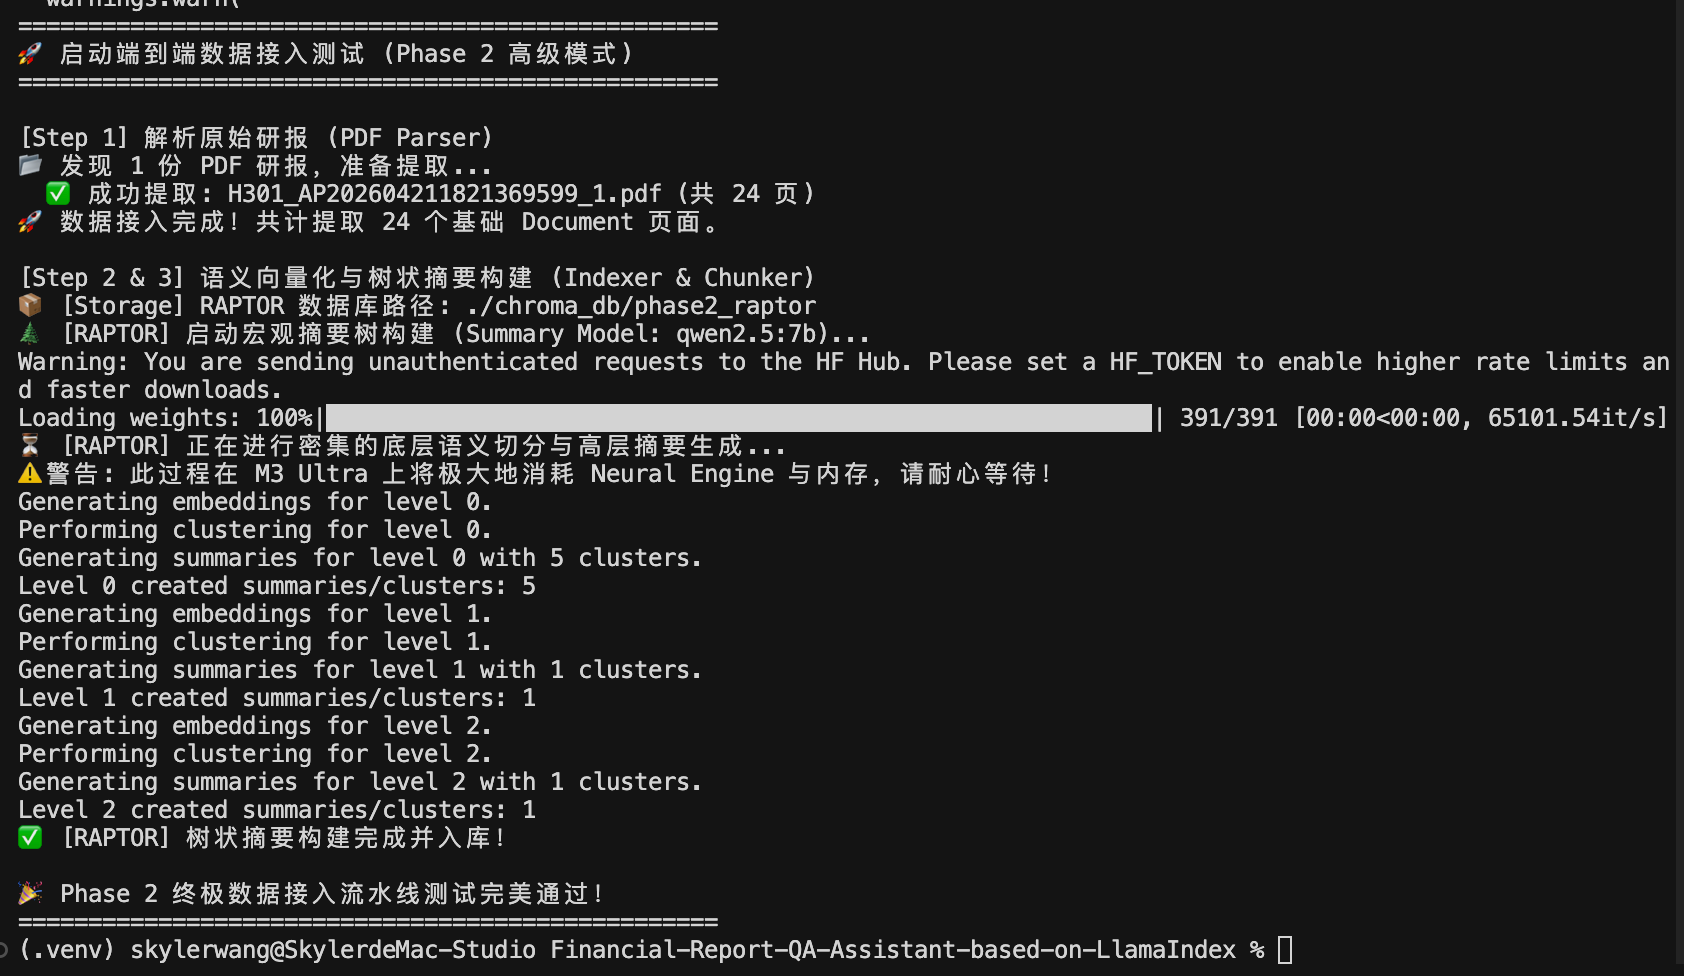
\includegraphics[width=0.6\textwidth]{../image/prompts/framework.png}
    \caption{Advanced Architecture (Semantic + RAPTOR)}
    \label{fig:framework}
\end{figure}

\begin{figure}[H]
    \centering
    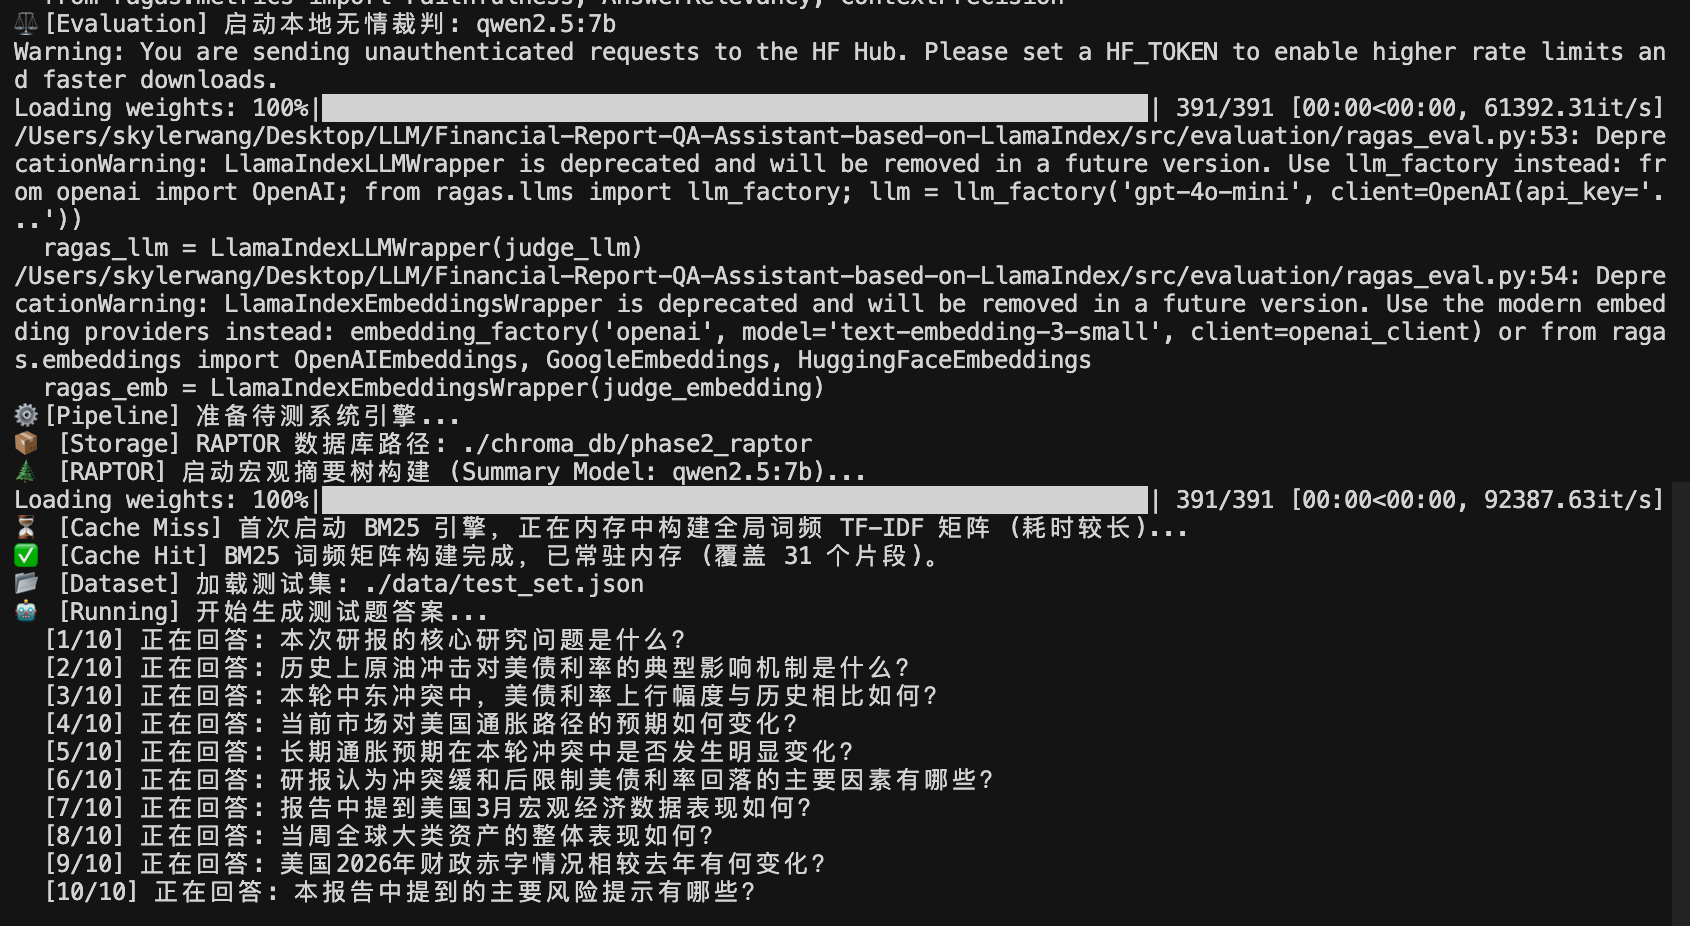
\includegraphics[width=0.6\textwidth]{../image/prompts/assess.png}
    \caption{Advanced Evaluation}
    \label{fig:assess}
\end{figure}

\section{Ongoing Work}

\subsection{Performance Optimization}
Currently optimizing system performance, including:
\begin{itemize}
    \item Optimizing vector index building and retrieval speed
    \item Improving chunking strategy to enhance information retrieval accuracy
    \item Optimizing large language model inference speed
\end{itemize}

\subsection{Feature Enhancement}
Currently enhancing system features, including:
\begin{itemize}
    \item Improving the accuracy of page-level citation tracking
    \item Adding multilingual support
    \item Enhancing understanding of tables and charts
\end{itemize}

\subsection{User Experience Improvement}
Currently improving user experience, including:
\begin{itemize}
    \item Optimizing frontend interface response speed
    \item Adding more interactive features
    \item Providing more detailed result explanations
\end{itemize}

\section{Challenges and Solutions}

\subsection{Challenge 1: PDF Parsing Accuracy}
Financial reports often contain complex formats, such as tables and charts,
which traditional PDF parsing tools struggle to extract accurately.

\textbf{Solution}: Adopted PyMuPDF for PDF parsing, combined with custom post-processing logic to improve parsing accuracy.

\subsection{Challenge 2: Long Text Processing}
Financial reports are typically long, and traditional RAG methods struggle to
effectively handle long text.

\textbf{Solution}: Adopted semantic chunking and RAPTOR tree-based summarization technology to decompose long text into manageable chunks and build hierarchical summary structures.

\subsection{Challenge 3: Comprehensive Evaluation}
How to comprehensively evaluate RAG system performance is a challenge.

\textbf{Solution}: Integrated RAGAS evaluation framework to evaluate system performance from multiple dimensions, including answer relevance, faithfulness, and completeness.

\section{Next Steps (Two-week Plan)}

\begin{enumerate}
    \item Complete performance optimization work to improve system response speed
    \item Complete feature enhancement work to add table and chart understanding
          capabilities
    \item Optimize UI design and user experience
    \item Deploy the system to production environment
    \item Collect user feedback to further improve the system
    \item Write detailed technical documentation
    \item Conduct comprehensive system testing and evaluation
\end{enumerate}

\section{Conclusion}

The Insight: Financial Report Analysis Engine project has made significant
progress, completing system architecture design and core module implementation.
By adopting advanced RAG technologies, the system can effectively analyze
financial PDF reports and provide accurate question-answering and analysis
capabilities.

Although some challenges were encountered during the project, they were
effectively addressed through team efforts and technological innovation. In the
future, we will continue to optimize system performance, enhance system
features, and improve user experience to provide a more powerful tool for
financial report analysis.

\end{document}